%!TEX root = ../thesis.tex
%*******************************************************************************
%****************************** Second Chapter *********************************
%*******************************************************************************

\chapter{Estado del Arte}

\ifpdf
    \graphicspath{{Chapter2/Figs/Raster/}{Chapter2/Figs/PDF/}{Chapter2/Figs/}}
\else
    \graphicspath{{Chapter2/Figs/Vector/}{Chapter2/Figs/}}
\fi

\section{Términos relacionados con el estilo de conducción}

El concepto de "Estilo de conducción" no tiene una definición estándar que sea aceptada en todo el mundo. Al contrario, este concepto involucra una serie de factores que aumentan su complejidad y complican su definición. Debido a esto se usarán los conceptos definidos por \citeauthor{8002632} \cite{8002632}.

\begin{figure}[htbp!]
\centering
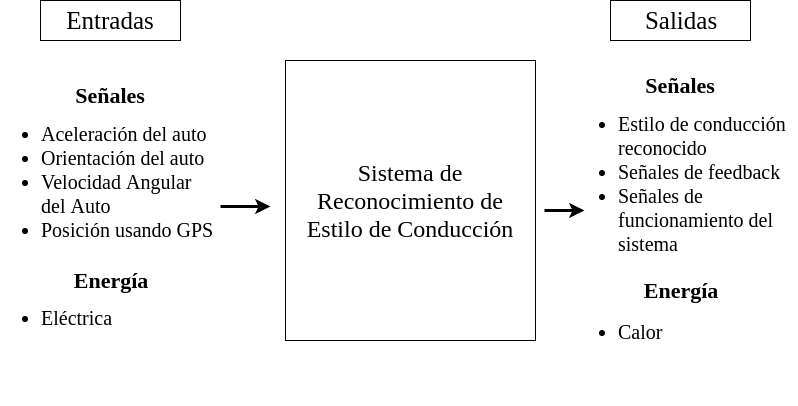
\includegraphics[width=0.8\textwidth]{Fig1}
\caption[Terminología estilo de conducción]{Terminología relacionada con el estilo de conducción \cite{8002632}}
\label{fig:1}
\end{figure}

Como se aprecia en la Fig~\ref{fig:1} \mynote{Traducir el gráfico} se entiende por un evento de conducción como las maniobras que se usan durante la acción de conducir, como por ejemplo: acelerar, desacelerar y girar.

De la misma manera, El patrón de conducción se define como el resultado de los eventos de conducción sujetos a condiciones de manejo, como el clima o el tipo de calzada. Este resultado se puede expresar como un perfil de velocidades. en el que están incluidos todos los datos que se pueden obtener partiendo de este perfil de velocidad, como por ejemplo: duración del viaje, velocidad promedio y demanda de potencia calculada.

La habilidad de conducción, es la habilidad que posee el conductor para controlar el vehículo. Este concepto se usa para diferenciar entre un conductor experimentado o profesional de un conductor promedio.

El estilo de conducción es más complejo de definir debido a que para algunos autores involucra factores subjetivos como la actitud del conductor, el humor o el cansancio. Para \citeauthor{6957822} \cite{6957822}, el estilo de conducción  es la manera en la que la tarea de conducción es realizada. Esto se traduce a la forma en la que el conductor opera el vehículo (Pedal de aceleración, timón, freno, etc.). Esto se diferencia de el patrón de conducción tan solo porque no se asocia con un recorrido en especifico sino con el conductor.

También se puede expresar el estilo de conducción en niveles de agresividad como \citeauthor{6294318} \cite{6294318}. Como la agresividad en los eventos de conducción esta asociada con un mayor consumo de combustible y a menor seguridad vial, definitivamente juega aun papel importante dentro del concepto de estilo de conducción. \mynote{Se debe definir cual es el concepto que se manejará en la tesis}

\section{Estado del arte según algoritmos usados}
Se procederá a mostrar las implementaciones e investigaciones desarrolladas en la actualidad clasificados según el tipo de algoritmo que se uso para la caracterización de el estilo de conducción

\subsection{Algoritmos basados en reglas}
Dentro de esta categoría se encuentran algoritmos de clasificación basados en reglas que comprenden el uso de lógica difusa, lógica difusa adaptativa y algoritmos de agrupamiento.

\citeauthor{6957822} \cite{6957822} desarrollo un sistema de reconocimiento de patrones de manejo online usando lógica difusa. Este sistema esta implementado usando {\it Matlab/Simulink}  y es totalmente paramétrico. Se puede configurar para ser usado en distintos tipos de vehículos.
El sistema determina a través de un Sistema de Navegación el tipo de calzada en el que se encuentra (Se distingue entre trocha, calles urbanas, carreteras pavimentadas y carreteras rurales). Esto lo realiza debido a que el tipo de calzada influencia en gran medida al estilo de conducción. Por ejemplo, en una trocha la mayoría de conductores manejarían a una velocidad suave para no dañar al vehículo.
Usando Lógica Difusa se definieron 3 niveles de estilo de conducción: {\it Normal, Confortable y Deportivo}. Se probó el sistema en una simulación y se obtuvieron los siguientes resultados: 68\% de clasificaciones correctas y solo 2\% de clasificaciones incorrectas (El otro 30\% pertenece a clasificaciones "diferenciales" que daban un resultado cercano al real)


